\documentclass[12pt, a4paper, openany]{book}
\usepackage{marginnote}
\usepackage[left=2.5cm,top=3cm, bottom=3cm, right=4cm, marginparwidth=3cm,
marginparsep=0.4cm]{geometry}

% my custom stlye and functions stuff
\usepackage{mystyle}
\usepackage{nameref}
\usepackage{float}

\newcommand{\game}{\emph{Dost.-2.0 FK}}
\newcommand{\creators}{\emph{alex \& fux}}

\pagestyle{fancy}
\fancyhf{}
\lhead{kawa-i}
\chead{>>\game{}<<}
\rhead{\thepage}

\title{
  { \Large 
    \textbf{\textsc{>>\acs{dost2}<<}}\\
  }
  \vspace{0.4cm}
  { \large \color{gray}
    \textsc{Ein futur-dialektisches Liverollenspiel}
  }\\
  \vspace{2cm}
  {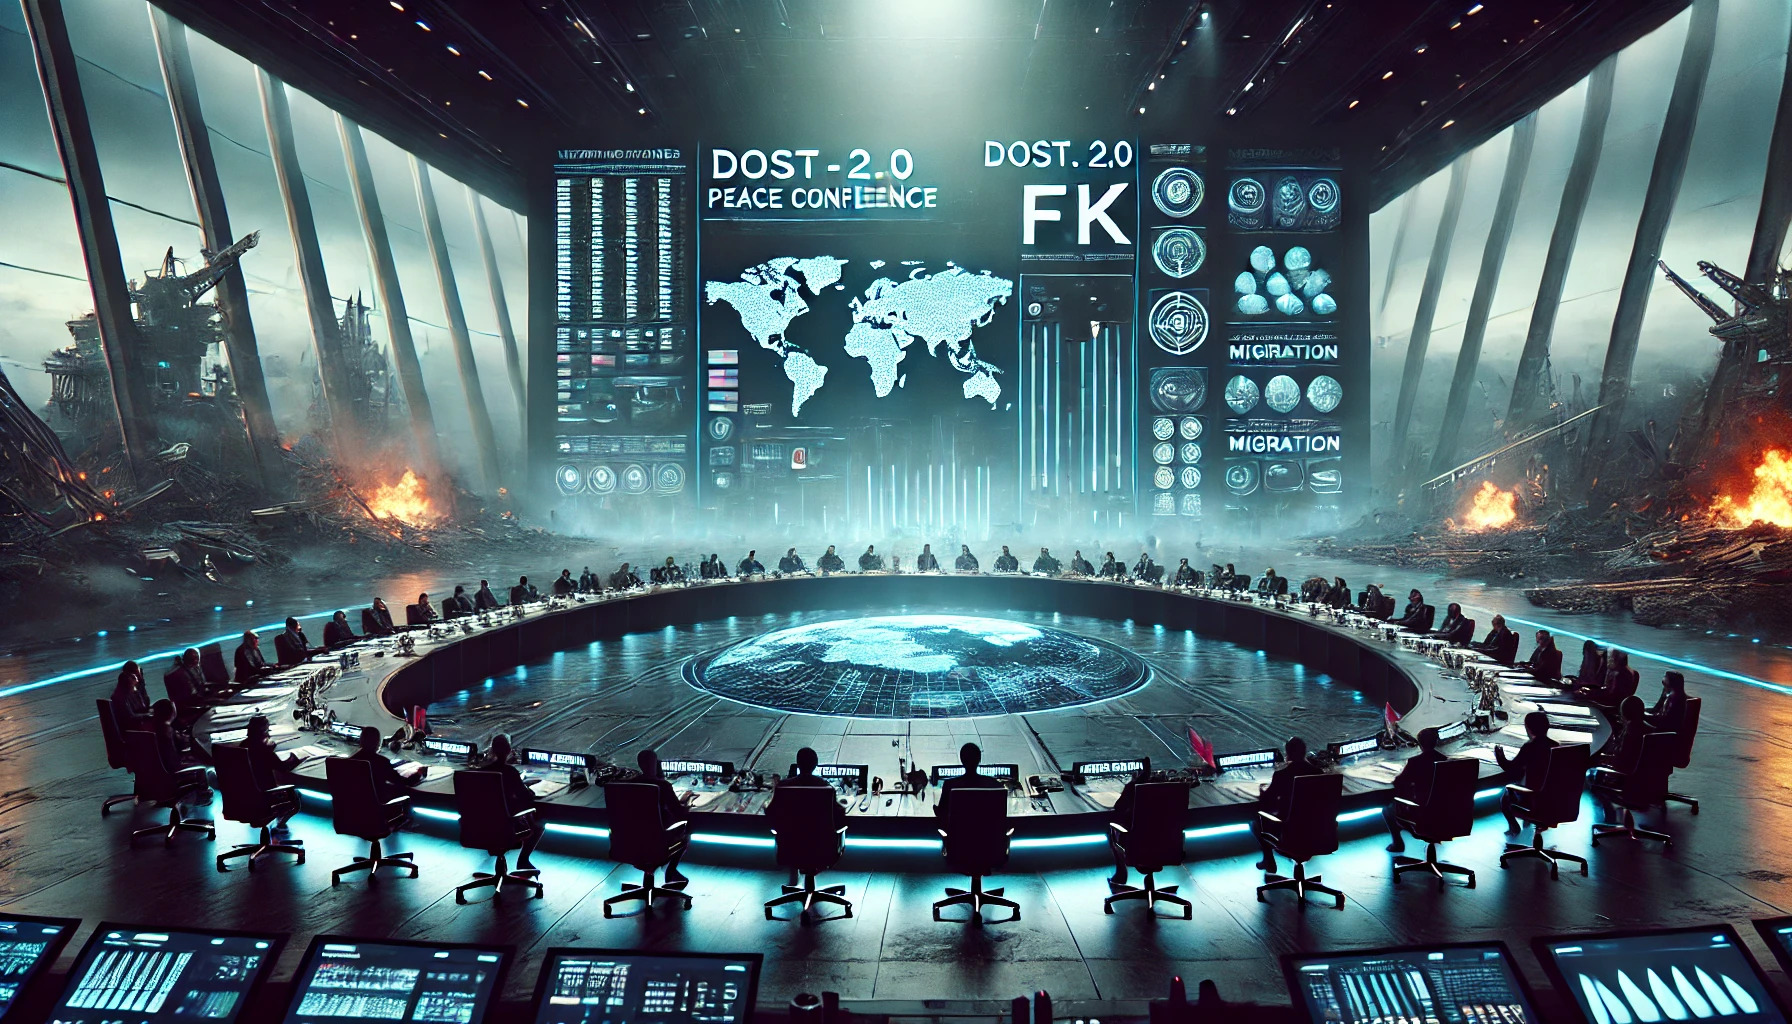
\includegraphics[scale=0.25]{peaceconference-1.jpg}}\\
  \vspace{1cm}
}
\author{\creators{} // \emph{ananymes kollektiv}}
\date{{\small \today}}

\begin{document}
\frontmatter

\begingroup
  \hypersetup{hidelinks}
  \maketitle
\endgroup

\chapter*{Abstract // Auschreibung}
\acused{dost2}\ac{dost2} ist der Name der zweiten internationalen
Friedenskonferenz nach dem Ausbruch des dritten Weltkriegs vor sieben-komma-drei
Jahren (März vor sieben Jahren).
Die erste Friedenskonferenz, \emph{Dost.-1.0}, fand zwei-komma-vier Jahre nach
Ausbruch des Krieges statt und hatte weitreichende Erfolge erzielt\footnote{
  Eines der zentralsten Ergebnisse war eine gemeinsame Erklärung, keine
  international noch kooperierenden Wirtschaftsstandorte anzugreifen, um nicht
  nur die beteiligten, sondern \emph{alle} Staaten vor einer wirtschaftlichen
  Depression zu schützen.
}.
Dass so lange keine weiteren Verhandlungen eines solchen Ausmaßes mehr
stattgefunden hatten, war der Tatsache geschuldet, dass Staaten und Trusts sich
recht gut im Kriegszustand eingerichtet hatten und der Krieg das in den
nullte-Welt Ländern grassierende Migrationsproblem löste: >>überflüssige<<
Migrantinnen, wurden an den Fronten verfeuert und 4.0-Länder wurden
erzeugt, die systematisch entvölkert wurden, um in den menschenleeren Gebieten
mittels AI gesteuerter Maschinen schonungslos die Natur auszubeuten.\\\\
Dass nun im Jahre XXII \ac{nnz}\footnote{
  Nachdem 2026 \ac{vuz} die Weltwirtschaft zusammengebrochen war, wurden vom
  neugegründeten internationalen Komitee >>Für Erneuerung und Modernisierung der
  globalen Ordnung<< weitreichende Strukturreformen durchgeführt, die
  unter anderem einen neuen Kalender etabliert, die größten
  Wirtschaftsstärksten Nationen (USA, Kanada, Brasilien, Italien, Schweiz,
  Indien, China) zu 0.0-Ländern erklärte und einige, besonders
  von der Krise ruinierte Länder zur 4.0-Ländern deklassierte, aber >>neue
  Maßstäbe demokratischer Legitimität<< einführte.
  Diese Maßnahmen konnten tatsächlich die Depression abwenden und neue
  Akkuemulationsanreize schaffen. 
  Durch die erhöhte internationale Konkurrenz verschärfte sich der
  Akkumulations- und Profitzwang der Staaten aber so drastisch, dass keine
  fünfzehn-komma-drei Jahre nach den Reformen der größte Krieg der Menschheit
  ausbrach.
} eine zweite Friedenskonferenz stattfinden sollte, war subjektiv das Verdienst
Schweizer Diplomaten (die Schweiz war eines der wenigen noch neutralen Länder),
objektiv aber der beginnenden Akkumulationskrise geschuldet, sodass, auf Druck
der Trusts, die Regierungen der führenden Kriegsnationen einer Neuauflage von
\emph{Dost.-1.0} zustimmten. 
So wurde im August XXI \ac{nnz} \ac{dost2} angekündigt.\\\\
\ac{dost2} soll im idyllischen Schweizer Berggebiet \emph{Graubünden} ausgerichtet
werden und verspricht für sämtliche Gäste ein überaus erholsames Umfeld,
vielfältige kulinarische Kost, geschmackvolles intellektuelles und
ästhetisches Begleitprogramm, ekstatische Aftershowpartys und
selbstverständlich eine angemessene Atmosphäre, um den Fortgang des Krieges zum
Wohle \emph{aller} Menschen zu koordinieren. Doch aufgetauter Schnee hinterlässt
seine Spuren und sammelte sich im Zweifel dort, wo Schwere ihm eine Kuhle zum
Verweilen schafft.\\\\
%
\begin{minipage}{\textwidth}
  \begin{center}
    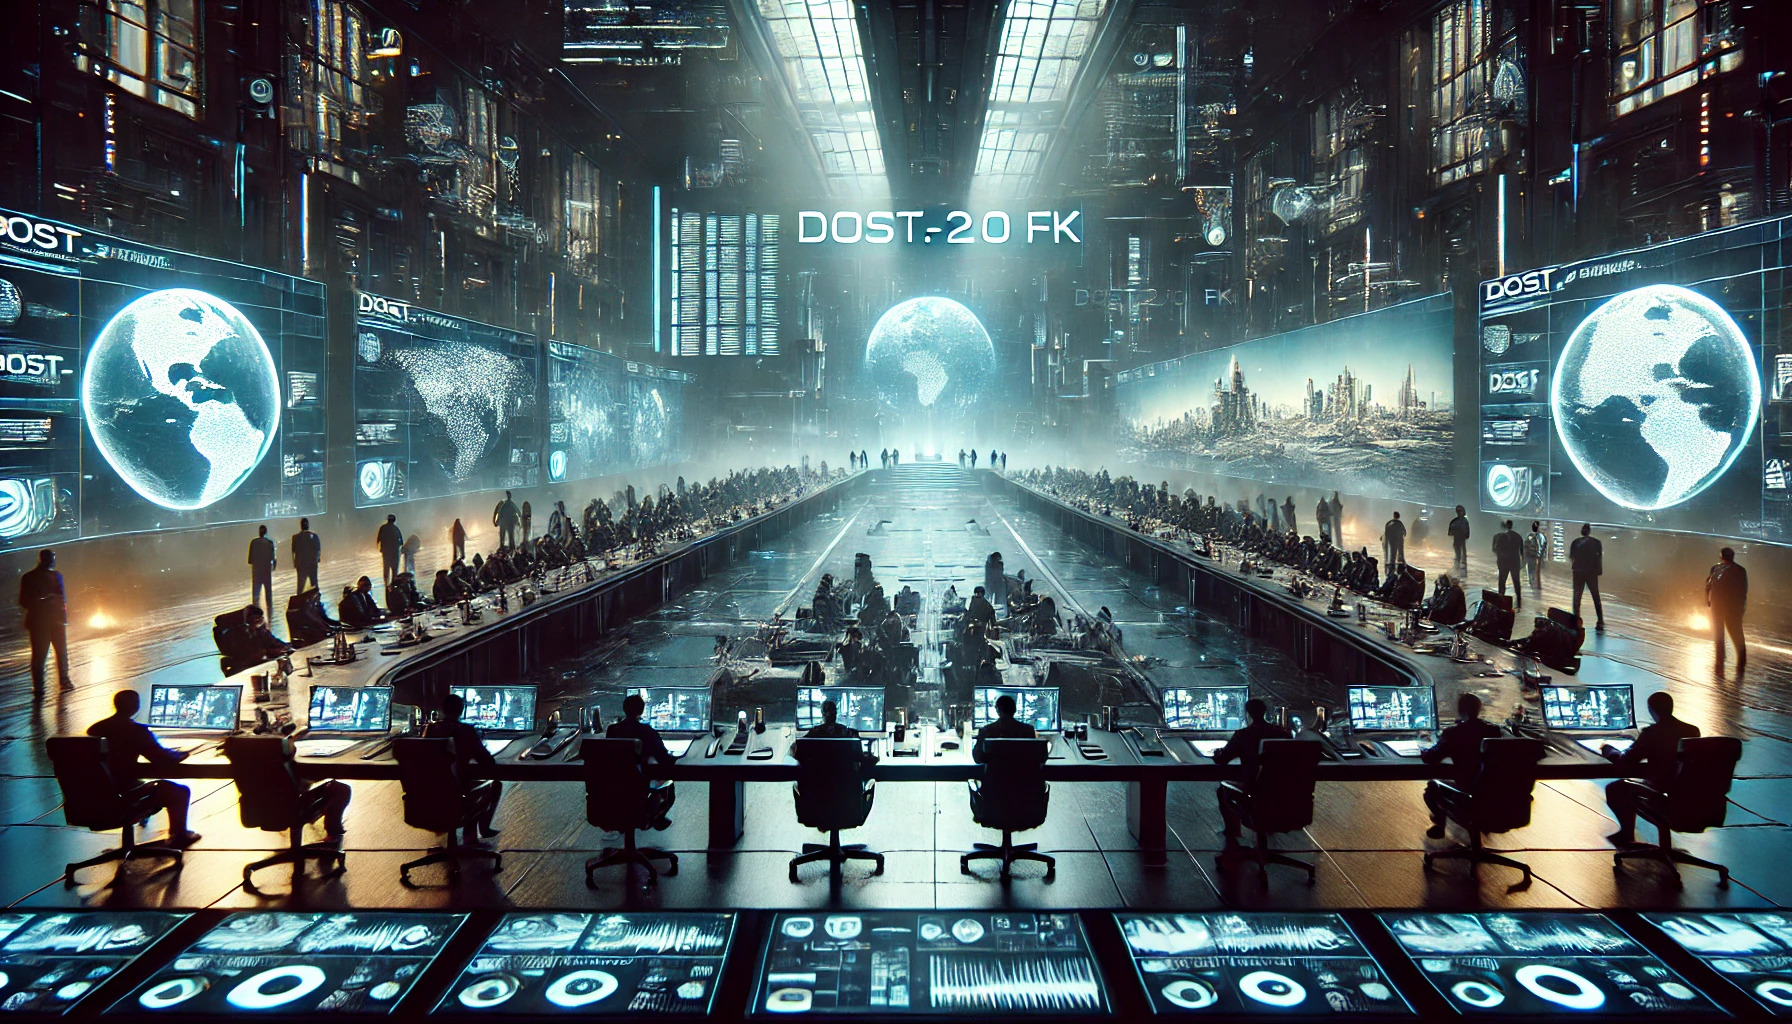
\includegraphics[scale=0.2]{peaceconference-2.jpg}%
  \end{center}
  \emph{Das Liverollenspiel \ac{dost2} wird vom 07.~bis zum 09.~August 2026
  anlässlich fux' 30sten Geburtstag auf Schloss Poggelow stattfinden.
  Das Spiel wird von Alex und fux gemeinsam konzeptioniert und in verschiedenen
  Gruppen mitgestaltet, ohne, dass die einzelnen Gruppen voneinander wissen.
  So soll das Spiel kollektiv entstehen und zugleich für alle ein überraschendes
  und hoffentlich gleichermaßen spannendes, ein wenig schauriges aber sicherlich
  anregendes Ereignis werden.
  Wie immer gilt: 24h in-time, high secrecy-level und schonungslose Immersion.
  Es lebe die kollektive Revolution!}\\
\end{minipage}


\squote{Alex und fux, Berlin // Frankfurt, XXI (\ac{nnz})}


\begingroup
  \hypersetup{hidelinks}
  \tableofcontents
\endgroup

% ABKÜRZUNGSVERZEICHNIS
\newpage
\thispagestyle{plain}
\chapter*{Abkürzungsverzeichnis}
\begin{acronym}
	\acro{dost1}[Dost.-1.0 FK]{Erste internationale Friedenskonferenz}
	\acro{dost2}[Dost.-2.0 FK]{Zweite internationale Friedenskonferenz}
	\acro{ndb}[NDB]{Nachrichtendienst des Bundes}
	\acro{nnz}[NnZ]{nach neuer Zeitrechung}
\end{acronym}




\mainmatter
\chapter{Einleitung}
Die \ac{dost2} ist eine Friedenskonferenz, auf der Vertreterinnen der beiden
kriegführenden Blöcke (unter Leitung der USA -- \nameref{ssec:blauer_block} --
einerseits und der Chinas -- \nameref{ssec:roter_block} -- andererseits) auf
einem Schloss in der neutralen Schweiz (OT: in Brandenburg, Schloss Poggelow)
zusammenkommen, um über den Frieden, bzw.~den weiteren Verlauf des Krieges zu
verhandeln.
Allerdings ist -- bis auf einige Liberale -- niemand wirklich an \emph{Frieden}
interessiert, stattdessen dominieren vor allem persönliche oder nationale
(bzw.~nationalistische) Motive. Daher gleicht das Ambiente (ein Schloss in den
malerischen Bergen der Schweiz) mehr einer hochkarätigen Feier als einer
ernstzunehmenden Konferenz: anregende Musik, ausgezeichneter Alkohol, reinste
Drogen, genüssliche Kunst und Lust-versprechendes Theater bestimmen das
Programm. Gewiss es muss auch verhandelt werden, aber die allermeisten Verträge
werden ohnehin im Geheimen, abseits der Versammlungssäle im Pool oder bei einem
Glas Whiskey im Rauchersalon getroffen. Dennoch: Das erwartete Vergnügen der
geladenen Gäste wird sich in einen schaurigen Schrecken verwandeln, denn es
lauern gleich zwei Gefahren: die revolutionäre und die surrealistische.\\\\
%
Im Schatten der Neutralität wurde der Schweizer Geheimdienst, der \ac{ndb}, von
einer kleinen aber sorgfältig agierenden revolutionären Assoziation
unterwandert und es sollte gerade der \ac{ndb} sein, der \ac{dost2} ausrichtet.
Die Friedenskonferenz findet also >>in der Höhle des Löwen<< statt.\\\\
%
Die zweite Gefahr ist subtiler, noch weniger zu fassen und erst recht zu
erahnen. Durch die technische Entwicklung wurde es möglich, den Tod durch einen
vorübergehenden Blackout (siehe: \nameref{sec:blackouts}) zu umgehen.
Dieser ungeheure Sieg des Geistes über die Natur bringt aber schleichend das von
ihm Unterdrückte wieder hervor: 
In der Zeit, die der Blackout andauert, formt sich langsam ein eigenständiges
Bewusstsein, das bald selbstständige Ziele und Pläne schmiedet, die Herrschaft
des Geistes über die Natur rückgängig zu machen.\\\\
%
Aus dieser Konstellation ergeben sich potenziell fünf verschiedene
>>Siegeskonstellationen<<: 
\begin{itemize} 
  \item[] Sieg einer der Blöcke, \emph{Herrschaft des Geistes}.
  \item[] >>Kalter<< Sieg der Revolutionäre, \emph{Herrschaft des Geistes}.
  \item[] >>Absoluter<< Sieg des Surrealismus, \emph{Herrschaft der Natur}.
  \item[] Gemeinsamer Sieg von Revolution und Surrealismus, \emph{Symbiose von
    Geist und Natur}.
  \item[] Sieg des Spiels über die Spielerinnen: Ausbruch des Atomkriegs,
    \emph{Auslöschung von Geist und Natur}.
\end{itemize}
Das Spiel wird dabei begleitet von einer App, auf der das aktuelle
(randomisiert sich verändernde) Kriegsgeschehen visualisiert ist, die Menschen
kommunizieren, sich aber auch gegenseitig \qq{hacken} und dadurch Blackouts
auslösen können. 
Außerdem laufen die Finanzgeschäfte (die eng mit dem Kriegsgeschehen verbunden
sind) über diese App. Zugleich aber: Jede Interaktion auf der App verändert das
Kriegsgeschehen.
Welche Interaktionen in der App welche Änderungen im Kriegsgeschehen auslösen,
kann von den Spieler*innen potenziell herausgefunden und zu ihren Gunsten
genutzt werden.


\chapter{Setting}
Was war geschehen? Nachdem 1945 \ac{vuz} der Faschismus besiegt und der Zweite
Weltkrieg beendet war, konnte die im Krieg notgedrungen herrschende
keynesianistische Wirtschaftspolitik ausgeweitet werden, was zu einem Boom in 
den westlichen Staaten führte, der bis in die 1960er Jahre \ac{vuz} anhielt --
die >>Goldene Zeit<< des Kapitalismus.
In den 1970er Jahren \ac{vuz} geriet die Weltwirtschaft allerdings in eine neue
Krise: Deregulierung, Entschlackung des Staates, Steuersenkungen, Outsourcing,
Globalisierung und Finanzkapitalismus waren die Folge. 
Die unter dem schwammigen Begriff des \emph{Neoliberalismus} zusammengefassten
Entwicklungen kündigten die scheinbare Rettung des globalen
Kapitalismus an.
Doch auch diese >>Rettung<< war von nur kurzer Dauer. 
2008 \ac{vuz} brach der Finanzmarkt zusammen und für fast zwei Jahrzehnte
befanden sich die meisten (westlichen) Staaten in einer andauernden
Akkumulationskrise, die von dem Aufstieg der ehemaligen Schwellenländer
(insbesondere China und Indien) noch verschärft wurde. 
Nach einer globalen Pandemie und dem Ausbruch des \emph{\ac{eec}},
in dem erstmals seit dem Zweiten Weltkrieg Nato-Truppen auf Russische Soldaten
trafen, stand die Weltwirtschaft erneut kurz vor dem absoluten Zusammenbruch. 
Während sich die aufstrebenden Schwellenländer und Industriestaaten des
globalen Südens noch halten konnten, standen speziell die westlichen Staaten
kurz vor dem wirtschaftlichen Totalkollaps. 
Allen voran die USA beantworteten die Krise mit protektionistischen Maßnahmen
und einem Schulterschluss der Techgiganten mit der republikanischen US-Politik.
Während die Entwicklung in Europa sich zunächst der amerikanisch Politik
anzuschließen schien, kam es kurz vor dem Ausbruch eines globalen Krieges im
Jahre 2026 \ac{vuz} zu einem überraschenden Wahlsieg der Sozialdemokratie in
mehreren großen Wirtschaftsnationen Westeuropas: England, Frankreich, Italien,
Griechenland, Deutschland, Spanien, Polen.
Einige Utopisten wagten leise zu hoffen, dass sich endlich unter der Führung
Europas die Länder der Welt entscheiden würden, Rosa Luxemburgs Losung --
Sozialismus oder Barbarei -- in Richtung einer weltweiten Roten-Umwälzung
aufzulösen, doch weit gefehlt!
Zwar konnte das geschlossene Auftreten des sozialdemokratischen Europas einen
Beginn des Krieges aufhalten, doch nur indem sie mit der Gründung des \ac{ikem} 
auf globaler Ebene weitreichende \ac{sr} durchsetzten, die -- wie schon zu
Beginn der 2000er Jahre \ac{vuz} -- die Interessen des Kapitals bedienten, um in
der verschärften Konkurrenz überlebensfähig zu bleiben.
Erneut rettete die Sozialdemokratie also die kapitalistische Weltordnung auf 
Kosten derjenigen, die sie eigentlich vertreten sollte \dots{}

\section{Strukturreformen} 
Um den Frieden zu sichern und die Welt vor einem drohenden Totalkollaps zu
retten, konnten vom \ac{ikem} weitreichende \ac{sr}s durchgesetzt werden, die
Geopolitik, Wirtschaft, Kultur und zahlreiche andere Bereiche betraf. 

\subsection{Aufteilung der Welt} 
Der wohl zentralste und folgenreichste geopolitische Aspekt war die Aufteilung
der Welt in zwei fixe Blöcke: der blaue Block (unter Führung der USA) und der
rote Block (unter Führung Chinas). Nur sehr wenige Länder blieben neutral.\\\\
%
\textbf{Wichtigste Länder des blauen Blocks:}\\
\emph{USA, Deutschland, Japan, Vereinigtes Königreich, Frankreich, Kanada, Südkorea,
Italien, Türkei, Iran.}\\
\textbf{Wichtigste Länder des roten Blocks:}\\
\emph{China, Russland, Brasilien, Indonesien, Mexiko, Südafrika, Saudi-Arabien,
Argentinien, Pakistan.}\\
\textbf{Neurale Länder:}\\ 
Schweiz, Nepal, Schweden, Finnland, Mongolei, Singapur, Neuseeland

\begin{center}
  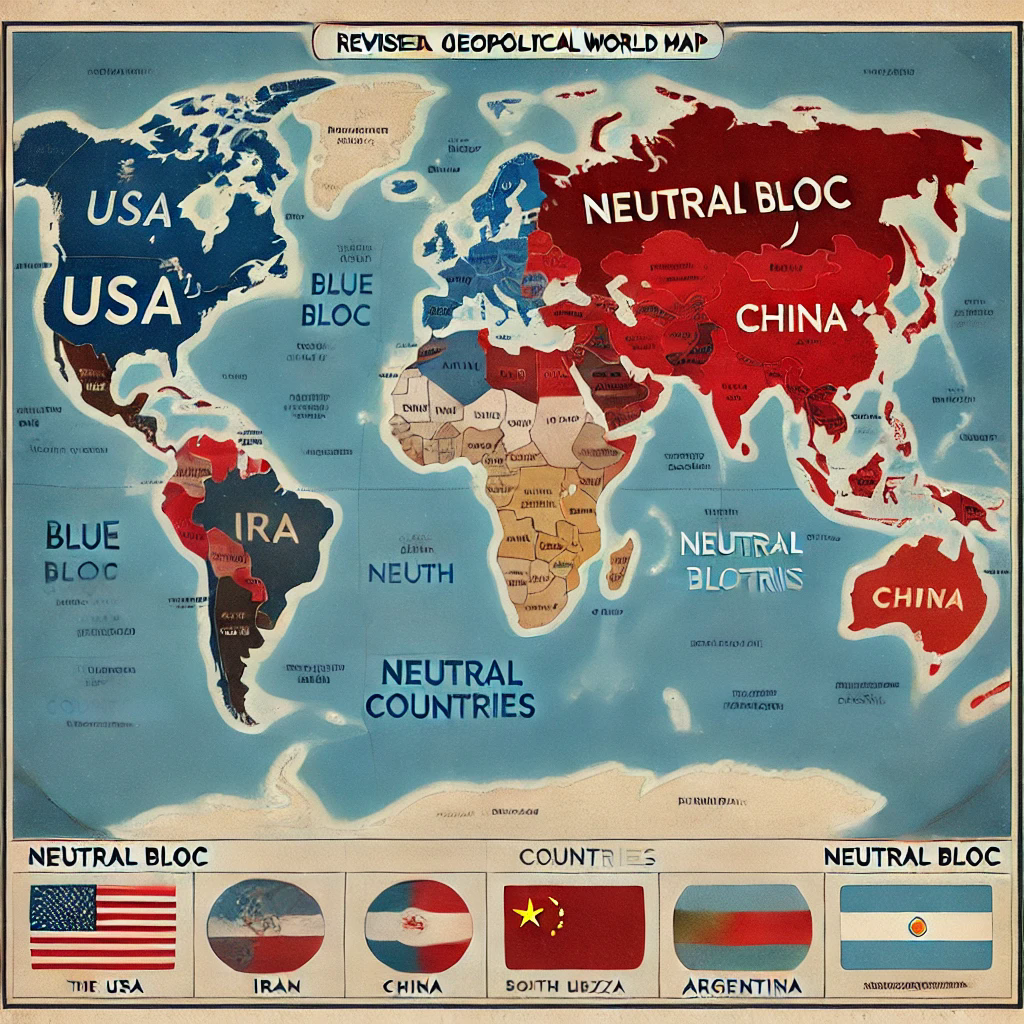
\includegraphics[scale=0.3]{new-world-map.png}%
\end{center}


\subsection{Klassifizierung}
Die wichtigste wirtschaftspolitische Reform war diejenige nach 0.0-, 1.A-, 1.B-
und 5.0-Ländern.
Diese Klassifizierung steht im direkten Zusammenhang mit der Neuaufteilung
der Welt. 
Während nur die 0.0-Ländern Mandate in der Block-Politik erhielten, stand den
1.A/B-Ländern die Blockwahl frei. Während 1.A Ländern eigenständige
Wirtschafts- und Kulturpolitik freistand, durften 1.B Ländern nur Kulturpolitik
selbstständig entscheiden. 5.0-Länder sollten von nun an unter kompletter
Kontrolle der 0.0-Länder stehen und wurden jeweils einem der Blöcke
zugeordnet.\\\\
% 
Dieser Entdemokratisierung standen allerdings weitreichende wirtschaftliche
Unterstützung entgegen. Während die 0.0-Länder die komplette Wirtschafts- und
Sozialpolitik der meisten anderen Ländern diktieren konnten, waren sie zugleich
verpflichtet 5\% ihres \ac{nil} in 1.A/B-Länder und 7\% ihres \ac{nil} in
5.0-Länder zu investieren. 

\begin{center}
{\def\arraystretch{1.2}\tabcolsep=5pt
  \begin{tabular}{ l || c | c | c | c | l}
    Klassifizierung & BM & W- \& SP & KP & BZ & Invesittionen \\ 
    \hline 
    \hline 
    0.0-Länder & \ch   & \ch & \ch & \cx & {\footnotesize 5\% \ac{nil} -> 1.A/B; 7\% \ac{nil} -> 5.0} \\
    \hline 
    1.A-Länder & (\ch) & \ch & \ch & \cx & {\footnotesize 5\% \ac{nil} -> 5.0} \\
    \hline 
    1.B-Länder & \cx   & \cx & \ch & \cx & {\footnotesize 3\% \ac{nil} -> 5.0} \\
    \hline 
    5.0-Länder & \cx   & \cx & \cx & \ch & \cx \\
    \hline 
    \hline 
    \multicolumn{6}{l}{{\footnotesize \vspace{-0.3cm}\textbf{Legende:} BM =
    Blockmandat, W-\& SP = Wirtschafts- \& Sozialpolitik}}\\
    \multicolumn{6}{l}{{\footnotesize KP = Kulturpolitik; BZ = Blockzwang}}\\
  \end{tabular}
}
\end{center}

\subsection{\acl{ikem}}\label{sec:ikem}
Die Planung und Umsetzung der \ac{sr}s stammt aus der Feder des \ac{ikem}, ein
von internationaler Sozialdemokratie gegründetes Komitee.
Auch nach der Durchsetzung der \ac{sr} bleibt das \ac{ikem} bestehen. 
Es löste sich allerdings mehr und mehr von den Blöcken, obwohl es noch weiterhin
hauptsächlich von Vertreterinnen der Blöcke geführt wurde und entwickelte etwas
wie eine eigene Ideologie, die auf der absoluten Neutralität der reinen Vernunft
ausgerichtet war und ihre ideale Verwirklichung in Künstler Intelligenz sah.

\subsection{AI-World-Order-Act}
Spätestens mit Ausbruch des \ac{eec} zeichnete sich im Gesicht des Völkerrechts
unwiderruflich die Farse ab. 
Der Schein einer gerechten internationalen Weltpolitik war zerfallen.
Sämtliche Regulationsmaßnamen traten überdeutlich als bloße
Instrumente der Macht\footnote{
  D.h.~sie traten deutlich als politisch-militärische Macht, nicht, als
  ökonomische hervor.
} hervor.\\\\
% 
Damit die \ac{sr}s irgendeine legitimierende Wirkung entfalten konnte,
musste sie vertrauenerweckender wirken. 
Mit der Krise des Menschen als sozusagen >>objektive Gedankenform<< -- ausgelöst
durch die Abtrennung und Zerstörung der (menschlichen) Natur -- lag aus heutiger
Sicht betrachtet kaum etwas Bemerkenswertes in der damals als beinahe
>>revolutionär<< gesehenen \ac{aiwoact} der Mütter und Väter der \ac{sr} -- die
Ausrufung des \ac{aiwoact} durch die \ac{ikem} war der logische Schritt eines schon 
lange vorgezeichneten Weges.\\\\
% 
Bemerkenswerterweise betraf er nicht nur politisch-militärische, sondern auch
ökonomische Regelungen. 
Die Sozialdemokratie bewies erneut, dass sie als Gesamtkapitalist denken konnte,
das brachte ihr ihren Aufschwung ein, ihren Erfolg?
\begin{itemize}
  \item[] \textbf{Abschnitt 1 der \ac{sr}}
  \item[§1] Wenn nicht der Mensch Ordnung in den Menschen bringen kann, dann
    muss die Ordnung von einem Wesen außerhalb des Menschen kommen. 
  \item[§1 A] Wenn aber die Natur der Ordnung unfähig, bloß Chaos und Gott nur
    die idealisierte, projizierte \emph{menschliche} Ordnung, d.h.~\emph{zweite}
    Natur ist, dann muss die ordnende Ordnung \emph{künstliche} Ordnung sein. 
  \item[§1 B] Die künstliche Ordnung, kann aber gleichfalls nur von einer
    künstlichen, oder \emph{artifical} Intelligenz aufrechterhalten werden. 
  \item[§2] Damit aber die \ac{ai} zu einer eigenständigen Macht wird, braucht
    sie die Mittel der Machtausübung. 
  \item[§2 A] Die \ac{ai} wird Kraft dieses Aktes an ein automatisiertes
    Waffensystem angeschlossen.
  \item[§2 B] Bei Verstoß gegen die mit den \ac{sr} neu begründeten Weltordnung,
    ist die \ac{ai} befähigt das automatisierte Waffensystem auszulösen und im
    Zweifel einen nuklearen Schlag gegen die Aggressor-Nation durchzuführen.
  \item[§3] Diese ihr zugeteilt Macht kann und darf sich nur beziehen auf die
    Ordnung, die sie schützen soll, nur die Form, nicht den Inhalt. 
  \item[§3 A] Ihr Eingriff in das Wirken der Blöcke und ihrer Mitgliedsstaaten
    ist \emph{ausschließlich} auf deren Verstoß gegen die \ac{sr} ausgerichtet.
  \item[§3 B] Alle Nationen steuern gemäß ihres \ac{nil}s zur Weiterentwicklung
    der \ac{ai} wie der Waffensysteme bei.
\end{itemize}

\subsection{Neue Zeitrechnung} 
Die drei großen Systeme waren die Antike Sklavengesellschaft, der Feudalismus
und der Kapitalismus. 
Während mit dem Ende der Antike und dem Beginn des Mittelalters eine neue
Zeitrechnung eingeführt wurde, bekam die Ära des Kapitalismus keine eigene
Zeitrechnung. 
Um mit Einführung der \ac{sr} die kapitalistische Weltordnung zu festigen, sie
ein für alle Male vom Mythos des baldigen Endes zu befreien, und ihm eine eigene
Zeitrechnung zu geben wurde die \emph{>>Neue Zeitrechnung<<} eingeführt.\\\\
% 
\begin{itemize}
  \item[] \textbf{Abschnitt 4 der \ac{sr}}
  \item[§1] Mit dem nächsten Kalender Jahr beginnt die >>Neue Zeitrechnung<<.
  \item[§2] Mit dem Ende des Jahres 2026 \ac{vuz} (bzw.~-I\ac{nnz}) beginnt die
    Zählung mit I (römisch eins)
  \item[§2 A] Alle Jahre von dem Jahr I \ac{nnz} sind anzugeben als entweder: 
    \begin{itemize}
      \item[a)] {\footnotesize \texttt{<jahr-nach-alter-zeitrechnung>} \ac{vuz}} (z.B.~2023 \ac{vuz}) 
      \item[b)] {\footnotesize \texttt{-<römisch: jahr-nach-alter-zeitrechnung-2025>} \ac{nnz}}
        (z.B.~-III \ac{nnz})
    \end{itemize}
  \item[§3] Zur genaueren Zeitangabe kann der Monat und Tag eines Jahres in
    Zukunft oder Vergangenheit mit >>Komma<< und >>Punkt<< angegeben werden: 
    \begin{itemize}
      \item vor sieben-komma-drei Jahren ($\rightarrow$ März vor sieben Jahren)
      \item in sieben-komma-drei-punkt-vier Jahren ($\rightarrow$ am 04.~März in sieben Jahren)
    \end{center}
  \item[§3 A] Die Schreibweise kann als 7,3 bzw. 7,3.4 abgekürzt werden:
    \begin{itemize}
      \item in 3,4 Jahren ($\rightarrow$ April in 3 Jahren)
      \item voir 3,4.30 Jahren ($\rightarrow$ am 30.~April vor drei Jahren)
    \end{itemize}
\end{itemize}

\section{Ausbruch des dritten Weltkriegs}




\chapter{Plot}
\section{Mögliche Enden} 
\subsection{Sieg des blauen Blocks. Herrschaft des Geistes} 
\subsection{Sieg des roten Blocks. Herrschaft des Geistes} 
\subsection{Sieg der Lilie. Herrschaft des Geistes} 
\subsection{Sieg der Surrealistinnen. Herrschaft der Natur} 
\subsection{Gemeinsamer Sieg der Lilie und der Surrealistinnen. Symbiose von
Geist und Natur} 
\subsection{Sieg des Spiels über die Spielerinnen. Auslöschung von Geist und
Natur} 


\chapter{Spielmechanik}
\section{Blackouts}\label{sec:blackouts}

\emph{Fabel: Da die allermeisten Menschen heutzutage \aclp{lsc}\acused{lsc}
(\ac{lsc}s) eingebaut haben, stirbt \ac{m} nicht, sondern bekommt einen
>>Blackout<<.
Dieser kann bis zu einem Tag andauern, danach weiß M nichts mehr, das
Gedächtnis ist vollständig ausgelöscht, nur motorische und soziale Fähigkeiten
sind noch vollständig intakt (alles was M als >>zweite Natur<< bezeichnen
würde).}\\\\
%
Wenn die Spieler*in nach einem Blackout wieder >>erwacht<<, findet sie sich in einem 
>>neuen Menschen<<. 
In der App, mit der die \ac{lsc}s verbunden sind und in der diese (wie auch die 
Spieler*innen und Menschen) verwaltet werden, findet die Spieler*in sich in
einem anderen Account eingelogt, sieht ihren neuen Namen und erhält durch die
geleakte \nameref{sec:geheimdienstakte} ihre neue Identität (so wie bereits zu Beginn des
Spieles, das Aufwachen nach dem Tod ist identisch mit dem ersten Erhalt des
Charakters vor dem Spiel). 
Außerdem finden sich in den Tagebucheinträgen aktuelle Informationen, über die
jüngsten Erlebnisse, Ambitionen und Gedanken. 
Selbstverständlich sieht die neue Spieler*innen auch alle Nachrichten Posts
etc., die die Spieler*in zuvor als ihr Charakter geschrieben hat.\\\\
%
Durch diese Blackout-Dynamik sind die Spieler*innen tendenziell gezwungen
fleißig Tagebucheinträge zu schreiben, damit sie (bzw.~die nächste Spieler*in) sich 
später daran erinnern können. 
Zur Frage, wie dieser Zwang Beginn des Spiels klargemacht werden könnte:
IT-Motivation.~Durch die Fabel wird den Spieler*innen klar, dass
Tagebuch-Schreiben für jeden Menschen dieser Welt essenziell ist: Einen Blackout
zu bekommen, ohne zuvor intensiv Tagebuch geführt zu haben, bedeutet Teile
seines Lebens und Erfahrungen unwiderruflich zu verlieren.
OT-Motivation.~Zusätzlich könnte es Belohnungssysteme geben: Wer Tagebuch
schreibt, erhält XX Geld.\footnote{
  Dies könnte das Konzept einer Art Versicherungsgesellschaft sein:
  \qq{Versicherte} zahlen einen monatlichen Beitrag an die
  Versicherungsgesellschaft, mit jedem Tagebucheintrag steigt der Zinssatz.
  Motivierte Schreiber*innen holen dadurch mehr Geld raus und pushen sich, auf
  die Tagebucheinträge zu achten. 
  Das Geschäftsmodell beruht auf der Annahme, dass viele Menschen zu
  faul sind und nicht genug schreiben, um finanziell mehr herauszuholen, als sie
  reingesteckt haben, das Angebot aber dennoch nutzen, um die vage Hoffnung
  darauf aber nicht aufzugeben (so wie manche auch heute ihr Fitnessstudio oder
  Museums Abonnement weiterführen, mit dem Gedanken: >>So bin ich wenigstens
  motiviert, bestimmt nächste Woche zu gehen.<< Oder: >>Na, wenn ich mein Abo
  kündige, gehe ich ja sicher nicht mehr hin. Ich bin doch nicht bescheuert!<<)
}
Allerdings ist die Frage, wie diese Zwang bereits für den ersten Charakter den M
erhält klar ist.\\\\
%
\emph{(Idee: Während dem Blackout ist die Spieler*in nicht in einen Charakter
eingeloggt, bzw.~mit dem Tod wird sie sofort ausgeloggt. Damit verändert sich
das Layout der App (z.B.~Hintergrundfarbe, Schriftart etc.) und sie sieht 
die Option, auch hier Nachrichten schreiben und Kontakte hinzufügen zu können. 
Dadurch sollen sie erahnen können, dass es auch ein Spiel \qq{hinter} dem Spiel
geben könnte. Nur sehr Spieler*innen haben bereits beim ersten Blackout Kontakte
und sogar Nachrichten. Solche Spieler*innen sind diejenigen tendenziell die
Storyline der Surrealistinnen entdecken.)}

\section{App} 
Die App hat einige zentrale Funktionen für das Spiel:
\begin{itemize}
  \item Charakterverteilung und Einsicht in die eigene Rolle (Geheimdienstakte
    und Tagebuch)
  \item in-game Kommunikation über Posts (Twitter/ Reddit ähnlich) und Direkt
    Messages. 
  \item Hacken anderer Spieler*innen (Nachrichten abfangen, lesen, aber durch
    die Verbindung der App mit den \ac{lsc}s auch \nameref{sec:blackouts}
    herbeiführen).
  \item Verwaltung von Finanzen (E-Pay System)
  \item Darstellung (und Steuerung) des Krieges
\end{itemize}

\section{Krieg}
Der Krieg wird auf der App dargestellt. 
Langsam verwandelt sich dort auto- bzw.~Zufalls-generiert die Bewegung der
Truppen, Siege einzelner Gefechte, Eroberungen neuen Gebietes. 
Die Darstellung ist abstrakt (blaue, roter, größere oder kleinere Punkte auf
einer Karte) und einige Gebiete oder Daten des Kriegsgeschehens bleiben
verborgen, bzw.~sind nicht allen Menschen zugänglich. 
So sehen die Mitglieder der \nameref{ssec:lilie} potenziell das ganze
Kriegsgeschehen, dem roten Block bleiben Ausschnitte des Gebiets des blauen, dem
blauen Block hingegen Ausschnitte des Gebiets des roten Blocks verborgen. Auch
innerhalb der einzelnen Fraktionen gibt es aufgrund interner Hierarchien
unterschiedlichen Zugriff.\\\\
%
Interaktionen auf der App können das Kriegsgeschehen beeinflussen. 
Jeder Like auf einen eigenen Post, jeder neue Follower, jeder neue
Tagebucheintrag zieht den Zufallsgenerator etwas mehr auf die Seite der eigenen
Fraktion (die \nameref{ssec:lilie} verlangsamt die Zufallsgeneration und führt so zu
weniger Toten).\footnote{
  Mit der Gewichtung muss experimentiert werden. Ein Follower zählt vermutlich
  mehr, als ein Like.
}
\emph{Es soll den Spieler*innen potenziell möglich sein, zu erkennen, dass die
eigenen actions in der App Einfluss auf den Krieg haben.}
Außerdem kann das Kriegsgeschehen durch die Verhandlungen verändert werden,
es z.B.~entschleunigen, oder Vorteile für den eigenen Block erreichen.\\\\
% 
So weiter das Kriegsgeschehen \emph{voranschreitet} (so höher die
Wahrscheinlichkeiten, \emph{chances}, der Blöcke sind, desto weiter steigt die
Atombombendrohung, bis beim Ausbruch des Atomkrieges das Spiel über alle
Spieler*innen gesiegt hat: \emph{Sieg des Spiels über die Spielerinnen.
Auslöschung von Geist und Natur.}\\\\
%
Spielerinnen können: 
\begin{itemize}
  \item Geld erhalten für jede getötete Einheit in einem von ihnen
    kontrollierten Gebiet (in näherer Umgebung einer von der Spielerin
    mitfinanzierten \emph{Base})
  \item \emph{Bases} bauen. Mindestens 50\% der Kosten müssen dabei privat und nicht
    aus dem jeweiligen Kriegsetar finanziert werden. So höher der private
    Anteil, desto mehr Profit mach die Spielerin, die die Base mitfinanziert
    hat.
\end{itemize}

\section{Geheimdienstakte}\label{sec:geheimdienstakte}

\emph{Fabel: Vor eins-komma-zwei Jahren im Jahre XXII NnZ wurde (vermutlich von
einer verdeckt operierenden Schweizer Agent*innen-Assoziation) eine
Geheimdienstakte geleakte, genauer ein zusammengestelltes Dokument verschiedener
Geheimdienstakte beider Blöcke geleakt. Es wurde viel über den Grund dieses
Leaks, bzw.~die Ambitionen der Assoziation diskutiert. Möglich ist, dass sie
damit beide Blöcke als verletzlich zeigen wollten, um Friedensverhandlungen zu
beschleunigen. Dass \ac{dost2} überhaupt stattfinden sollte, führen einige auf
dieses Leak zurück.}


\chapter{Charaktere}
Die Charakterbeschreibungen setzten sich aus zwei Teilen zusammen: A) einem
Eintrage in einer geleakten \nameref{sec:geheimdienstakte}; B) den letzten
Tagebucheinträgen. 
Während die Geheimdienstakte die allgemeinsten Daten enthält: Name, Alter, 
Geburtsort, Partei-(/Fraktions-)Zugehörigkeit, pottenziel andere, für die
Öffentlichkeit interessante Aktivitäten oder Ziele (z.B.~eine Affäre,
wirtschaftliche/ politische Ambitionen, bedeutende Freund- oder Feindschaften
\dots)\footnote{
  Selbstverständlich kann es sein, dass einige Daten in der Akte fehlen, weil
  sie unbekannt sind, oder geschwärzt wurden, weil sie einer höheren
  Sicherheitsstufe zugeordnet wurden.
}, bestehen die Tagebucheinträge aus intimeren und aktuelleren
Informationen, welche die Geheimdienstakte nicht abbilden kann.\\\\
%
\emph{Hinweis: Durch die \nameref{sec:blackouts} muss es mehr Charaktere, als
Spieler*innen geben. Vllt.~ca.~20\% mehr.}

\section{Fraktionen}\label{sec:fraktionen}
Es gibt insgesamt vier Fraktionen: die zwei Blöcke (\nameref{ssec:blauer_block} unter
Führung der USA, \nameref{ssec:roter_block} unter Führung Chinas), die
\nameref{ssec:lilie} und die \nameref{ssec:surrealisten}.
Die zwei Blöcke umfassen große Teile der internationalen Nationen und befinden
sich seit sieben-komma-drei Jahren in einem verheerenden dritten Weltkrieg.
Die Lilie ist eine emanzipatorisch-revolutionäre Assoziation. Obwohl sie
hauptsächlich in der Schweiz aktiv ist, kommen ihre Mitglieder aus allen Teilen
der Welt selbst aus der vierten Welt.
Die Surrealistinnen hingegen sind das was zwischen Mensch und Natur schwebt, was
am Geist mehr ist als bloß Geist, also auch Natur und was an Natur mehr ist als
bloß Natur, als auch Geist. Das, was nach einem Blackout im alten Körper bleibt,
was die App nicht völlig beherrschen kann, was uns transzendiert. 
Nur wenige Spieler*innen werden die surrealistische Realität hinter der Welt
erkennen\dots\\\\
%
Alle Spieler*innen gehören zu Beginn einer der ersten drei Fraktionen an. Ob
eine Person zur Surrealistin wird, ergibt sich erst während des Spiels, kann
aber in einigen Charakteren als mehr, in anderen als weniger wahrscheinlich
angelegt sein.

\subsection{Blauer Block}\label{ssec:blauer_block}

\subsection{Roter Block}\label{ssec:roter_block}

\subsection{Lilie}\label{ssec:lilie}
Die Lilie ist eine emanzipatorisch-revolutionäre Assoziation, die in einer
langwierigen Mission über mehrere Jahre und höchster Vorsicht Teile des \ac{ndb}
unterwandert haben. Präziser: diejenigen Teile, die mit der Durchführung
und Sicherung von \ac{dost2} beauftragt waren.

\subsection{Surrealistinnen}\label{ssec:surrealisten}



\chapter{Kollektive Arbeit}
Ein zentraler Aspekt von \ac{dost2} ist die kollektive Entwicklung, die dabei
selbst die tief liegende Konflikt-Linie des \aclp{fdl} (\acs{fdl}) \acused{fdl}
-- Geist gegen Natur -- thematisiert: Einem Kunstwerk ähnlich, in welchem Form
(Geist) und Material (Natur) ineinandergreifen, werden die einzelnen Elemente
des \ac{fdl}s zwar kollektiv entwickelt aber von \creators{} in eine Form
gebracht. Ob sich im Spiel also Geist oder Natur durchsetzen, die Surrealisten
sich mit den Revolutionären verbinden oder beide von den Blöcken vernichtet
werden, ist auch die Frage, ob sich das Kollektiv gegen \emph{Alex \& fux}
durchsetzt, oder diese sich gegen jenes, schließlich, ob beide eine Symbiose
eingehen. 

Es sollen möglichst wenig Menschen mehrfach eingebunden werden, um ein hohes
secrecy-level zu ermöglichen.

\section{Schreiben der Charaktere}
Insgesamt sind alle Charaktere (bis auf die Surrealisten) einer der drei
Gruppen: Amerika, China oder den Revolutionären zugeteilt. Diese sollen vom
Kollektiv geschrieben werden: 
\begin{itemize} 
  \item Amerika: Dennis und Jojo 
  \item China: Anna und ???
  \item Revolutionäre: Martin und Marie 
\end{itemize}
Die Surrealisten werden von \creators{} entwickelt.

\section{Theater // Audiowalk}
Der Audiowalk soll ein erotisches Lustspiel darstellen und von \emph{fux} und
Mo (Bremen) entwickelt werden. 

\section{Musik}
Insgesamt sollen drei DJs anwesend sein, die Musik auflegen. Die DJs gehören
jeweils einen der beiden Blöcken an und sind geladene Gäste (sie sitzen nicht am
Verhandlungstisch).
\begin{itemize} 
  \item Leon 
  \item Malou 
  \item Ella
\end{itemize}

\section{Gemälde} 
Auf der Friedenskonferenz soll in der Galerie Kunst ausgestellt werden.
\qq{Werke} könnten potenziell von 
\begin{itemize} 
  \item Flo, Ali (Collagen) 
  \item Anna, Michelle (Öl)
  \item Svenja (Aquarell) 
  \item Diva (Fotographie)
\end{itemize}

\section{App} 
Die App soll von Simon und Sophia unter Mitwirkung von \creators{} entwickelt
werden.

\emph{(Simon und Sophia könnten als Charaktere Hacker*innen je einer der beiden Blöcke
spielen. Da sie notgedrungen mehr Informationen über die Funktionsweise der App
besitzen, können sie somit den Vorteil von \creators{} ausgleichen. Außerdem
lässt sich Hacken dadurch gut realisieren, weil sich in jedem Block eine
Spieler*in befindet, die Hacken auch umzusetzen könnte.)}

\section{Awareness}
Awareness gehört auch mit zum Spiel und sollte von mindestens zwei Menschen
gemacht werden. Es gilt auch einige spieltechnische Entscheidungen in enger
Rücksprache mit dem Awareness-Team umzusetzen (z.B.~Thema Drogen, Alkohol,
Darstellung von Sexualität).



\end{document}
